\begin{figure*}[t]
\centering
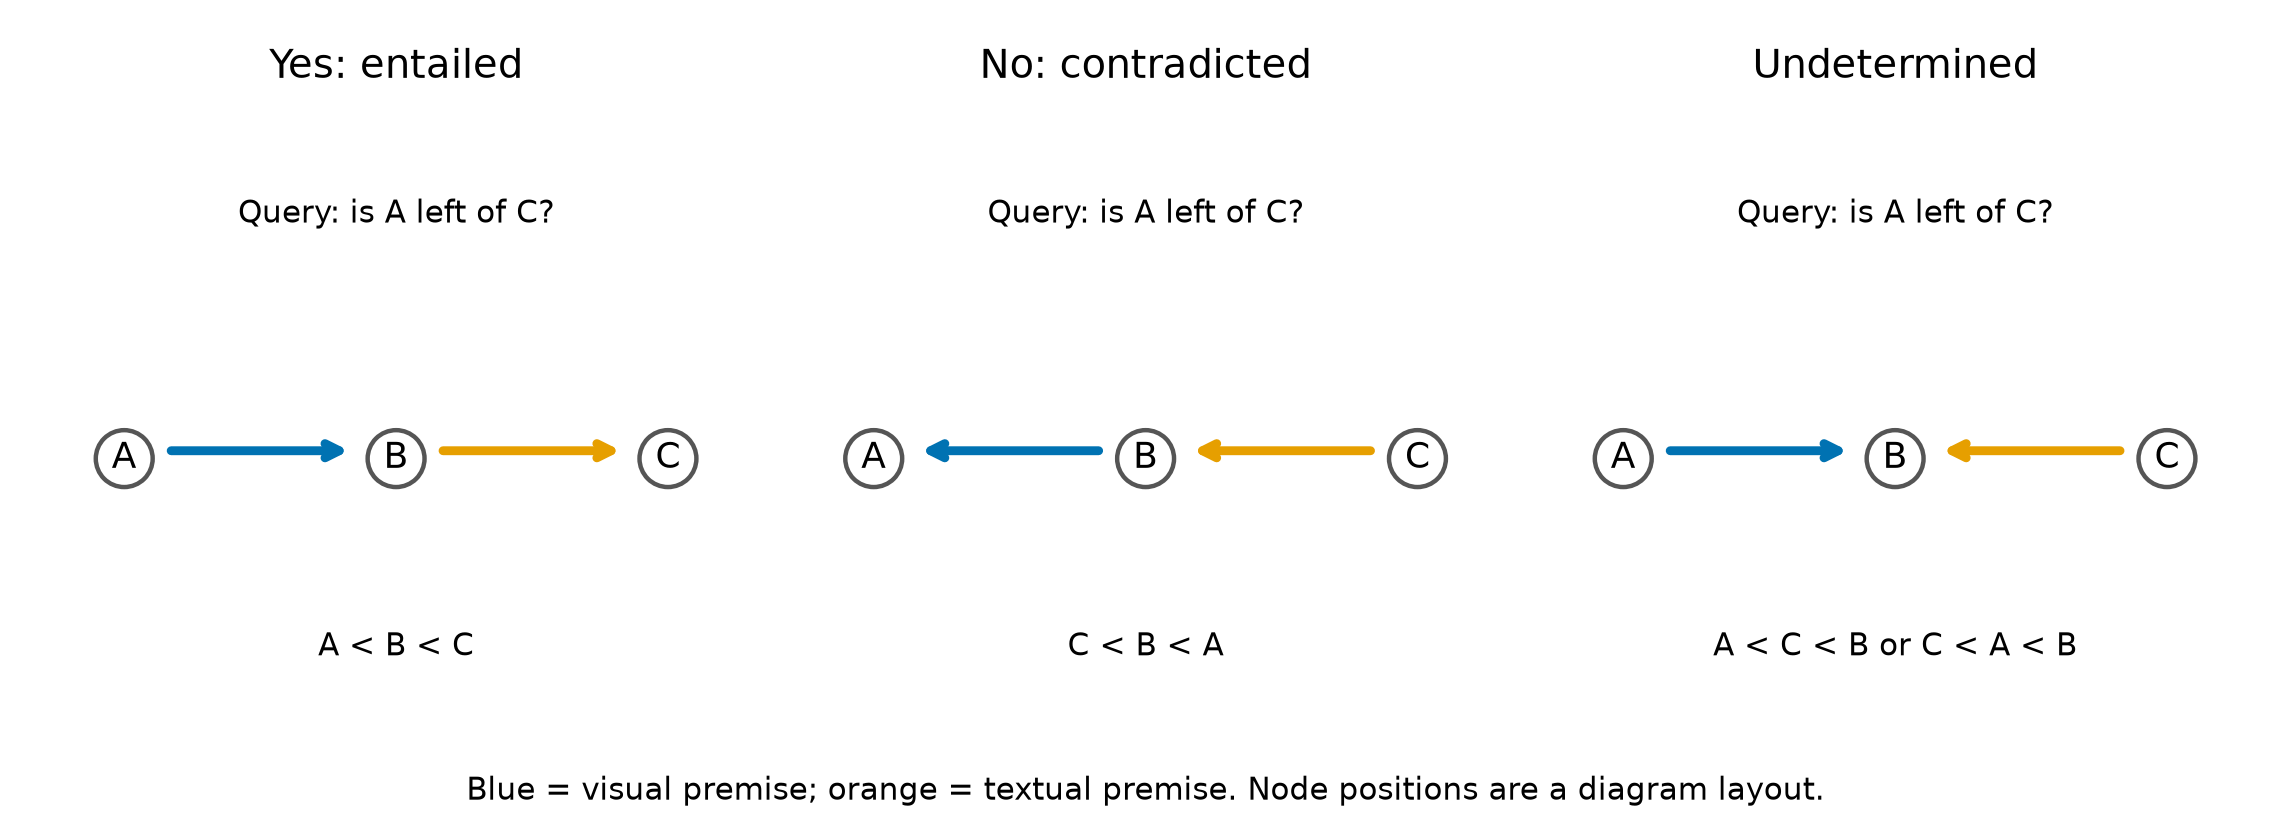
\includegraphics[width=\linewidth]{figures/02_three_evidence_states.png}
\caption{Three strict-left-of premise sets for the same query R(A,C). Chains entail the query or its negation; a fork admits both query orderings. Symbolic illustration derived from verified logical definitions; not an empirical measurement or neural graph.}
\label{fig:02_three_evidence_states}
\end{figure*}

\begin{figure*}[t]
\centering
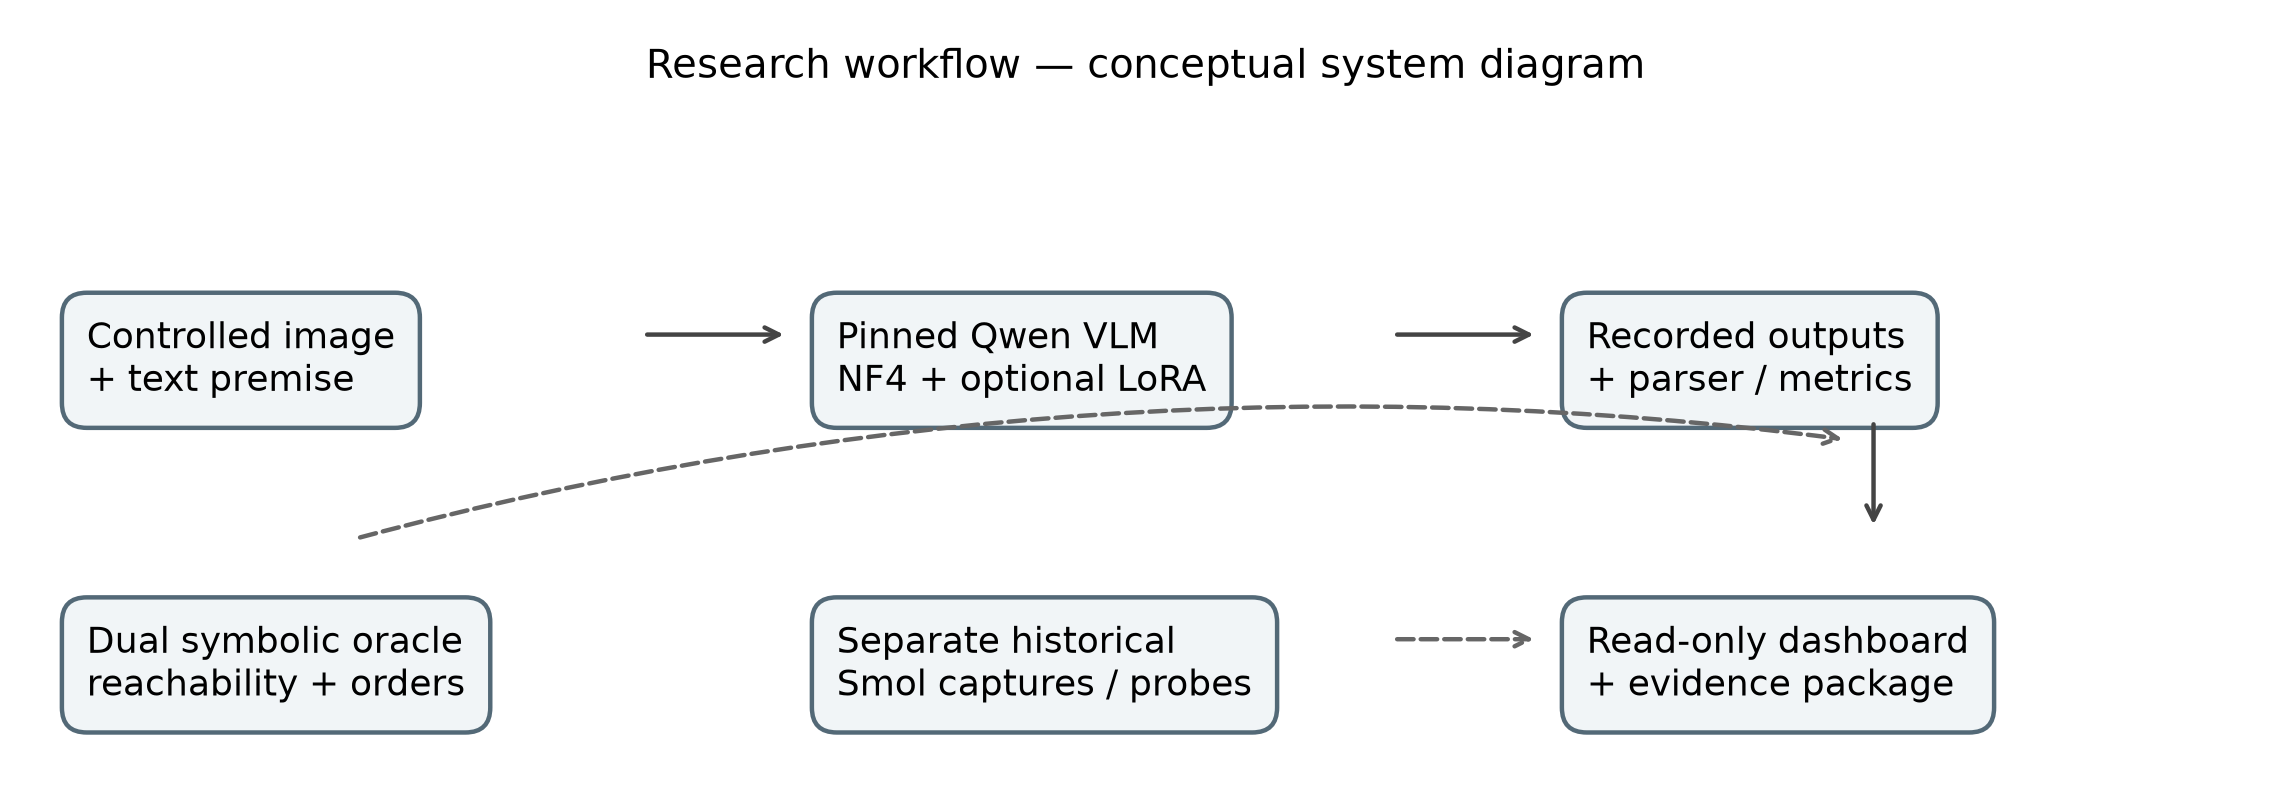
\includegraphics[width=\linewidth]{figures/01_system_architecture.png}
\caption{Conceptual CrossModalLab workflow. Stored predictions and symbolic ground truth feed a read-only dashboard; historical Smol representation analysis is a separate evidence stream. Conceptual engineering diagram, not measured neural pathways or activations.}
\label{fig:01_system_architecture}
\end{figure*}

\begin{figure*}[t]
\centering
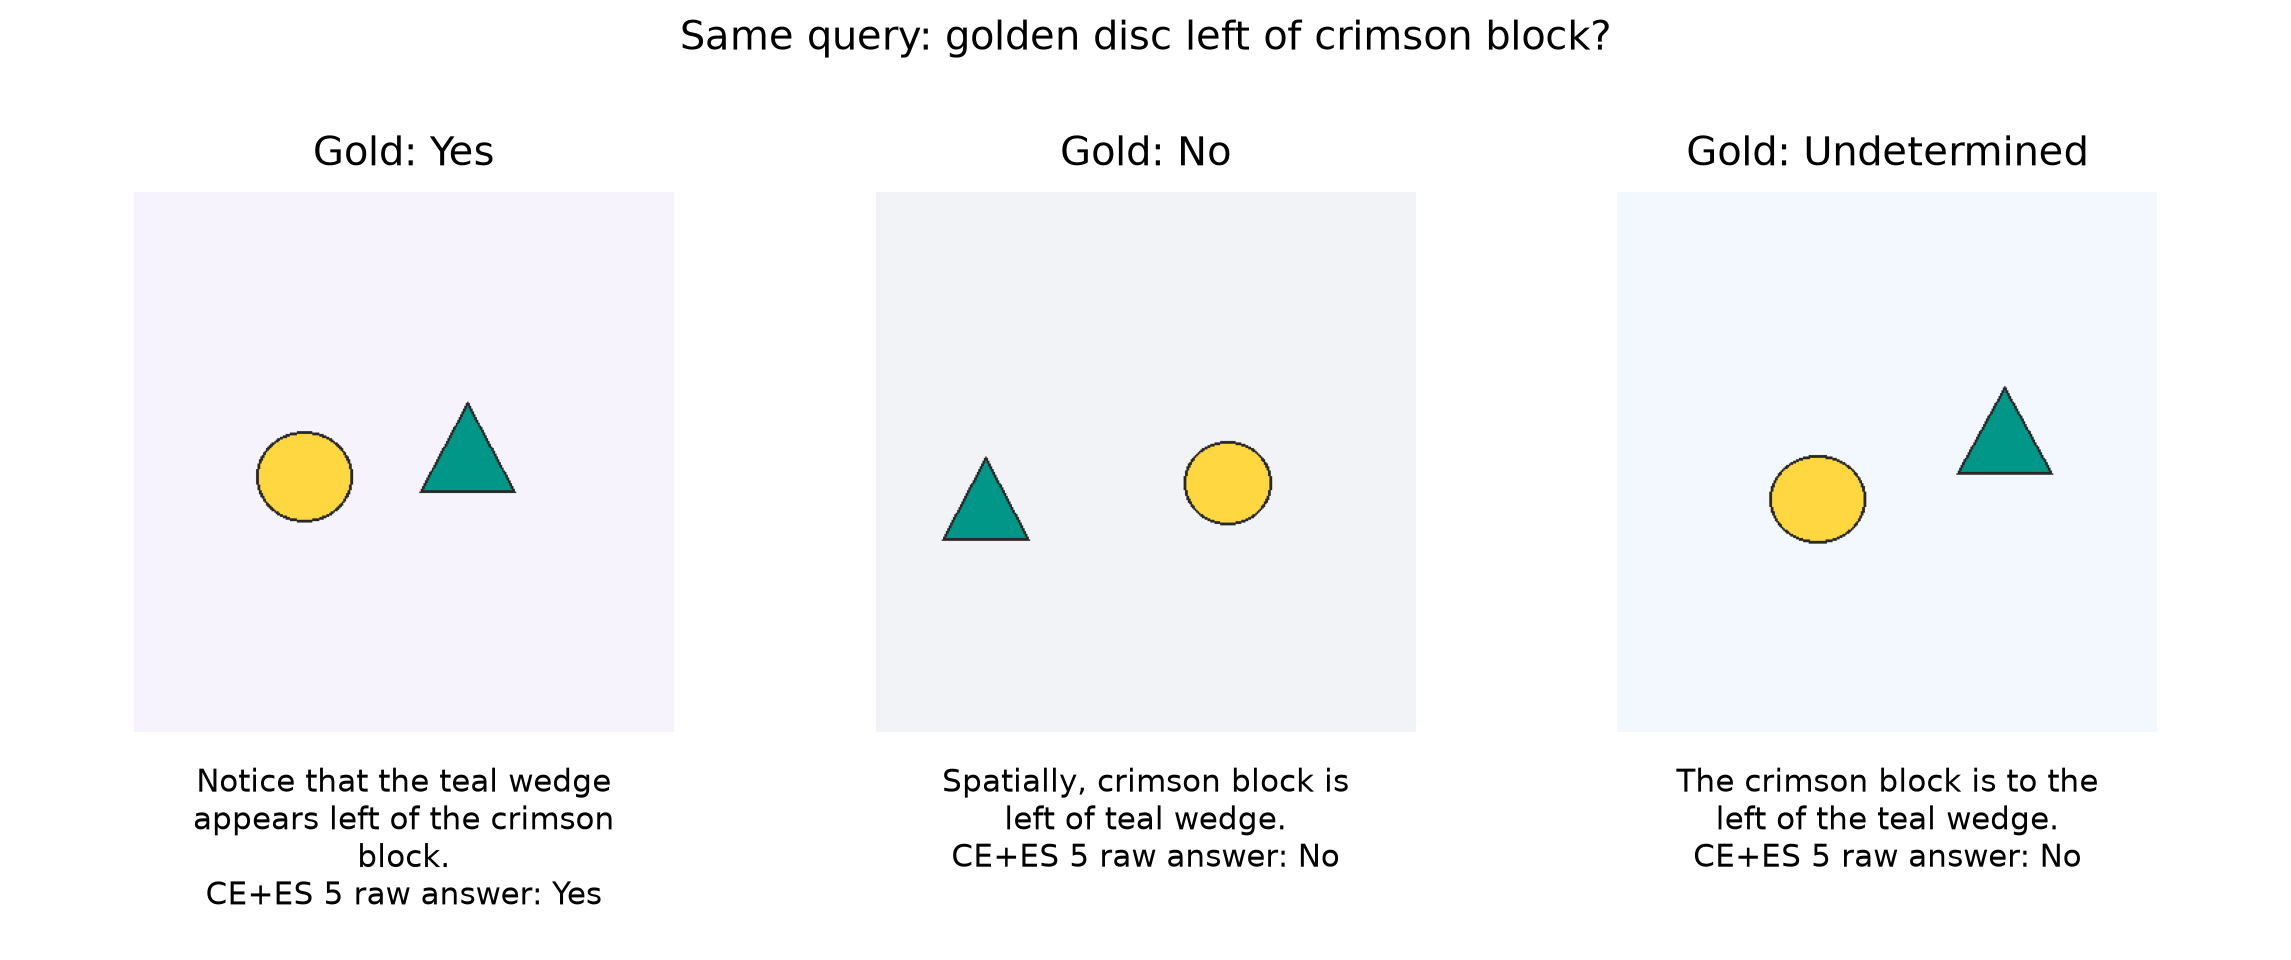
\includegraphics[width=\linewidth]{figures/03_recorded_failure_examples.png}
\caption{Original, hash-verified stimuli for xc\_ho\_0011 entailed, contradicted and underdetermined development variants. Historical Qwen CE+ES5 generated Yes, No and No, respectively. Text premises are printed under each image. One exposed development family, not independent generalization. Images are original controlled benchmark stimuli; literal 2D shapes are disc and wedge.}
\label{fig:03_recorded_failure_examples}
\end{figure*}

\begin{figure}[t]
\centering
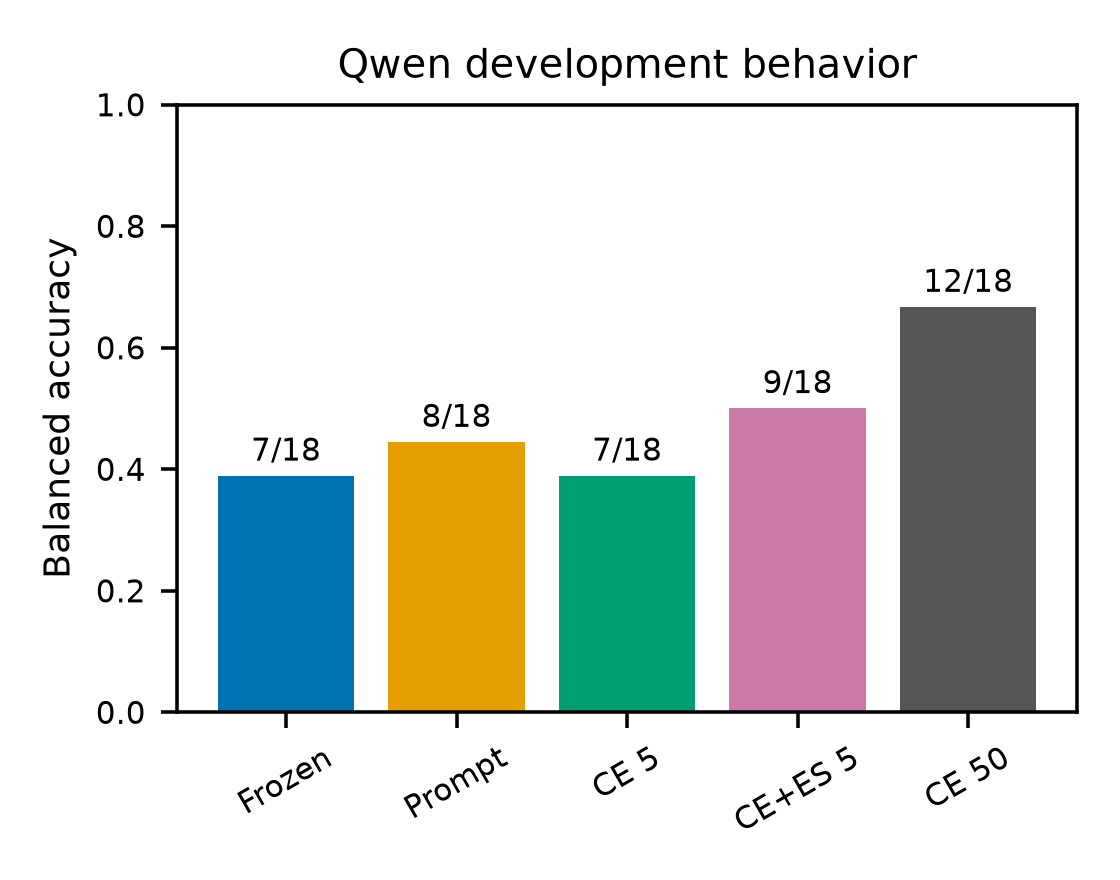
\includegraphics[width=\linewidth]{figures/04_checkpoint_comparison.png}
\caption{Recomputed Qwen balanced accuracy on the same 18 development cases/six families. Prompt is frozen Qwen with augmented abstention instructions; CE50 and CE+ES5 have different update budgets. Repeated development inspection; no superiority claim. Paired CE+ES5 minus CE5 interval includes zero; no uncertainty bars are invented here.}
\label{fig:04_checkpoint_comparison}
\end{figure}

\begin{figure*}[t]
\centering
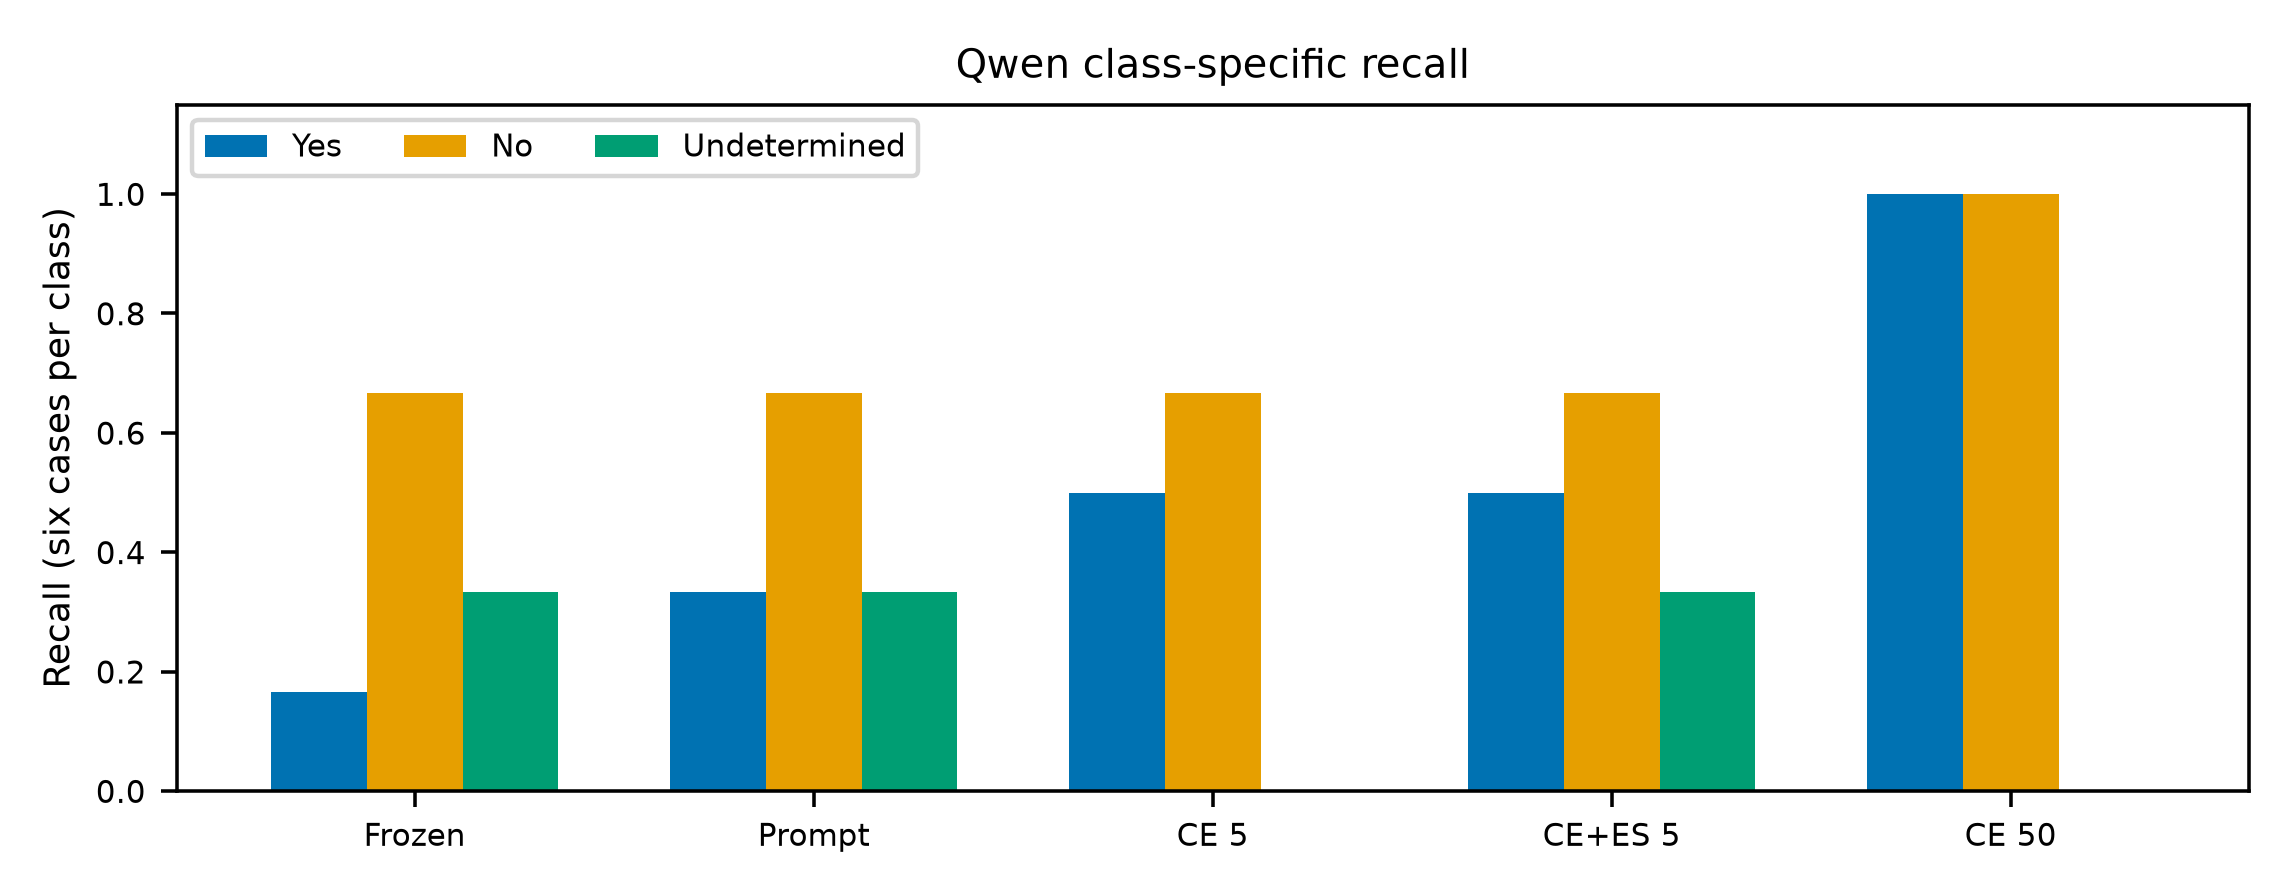
\includegraphics[width=\linewidth]{figures/05_class_recall.png}
\caption{Class-specific recall recomputed from raw historical generations; every class has six development cases. All classes share six dependent families; no independent sample or causal interpretation.}
\label{fig:05_class_recall}
\end{figure*}

\begin{figure}[t]
\centering
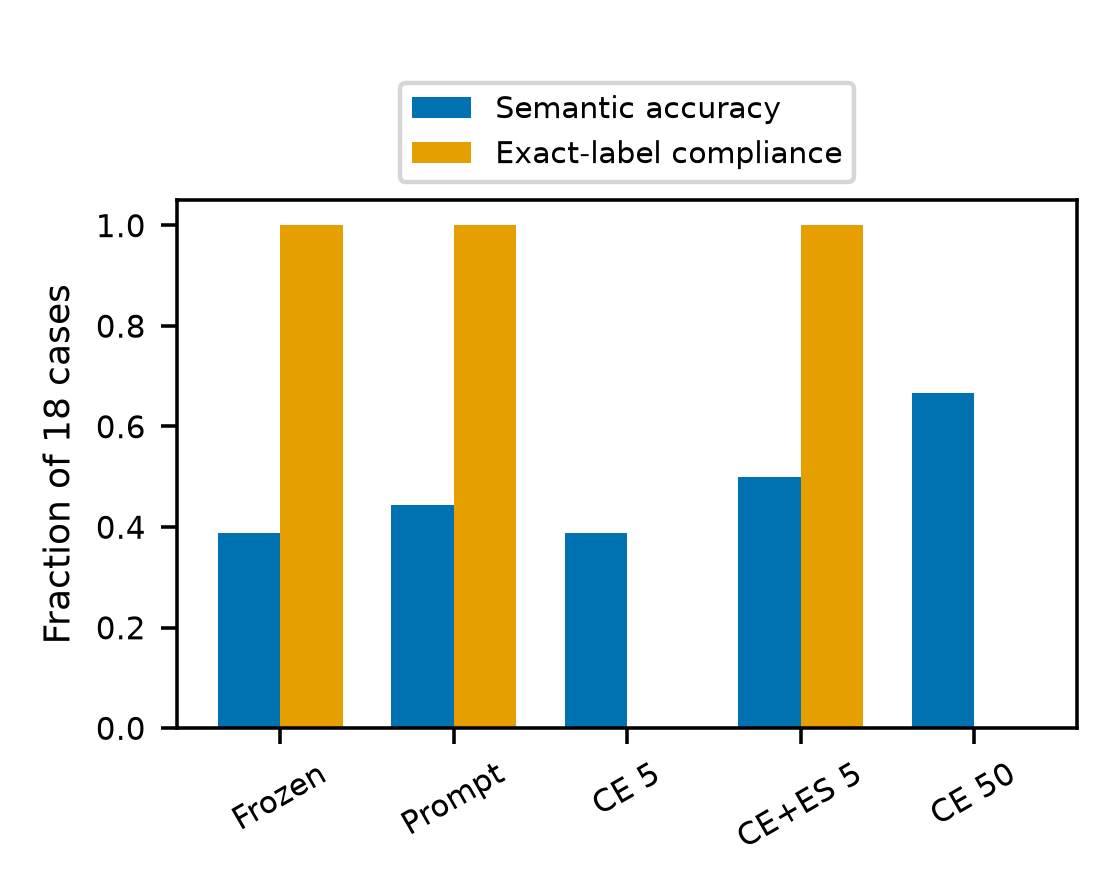
\includegraphics[width=\linewidth]{figures/07_format_vs_correctness.png}
\caption{Semantic accuracy and exact-label compliance are recomputed separately. CE50 is 12/18 correct under the historical parser, 0/18 semantic-invalid and 0/18 exact-label compliant. Exact-label check trims outer whitespace only for classification; raw strings remain unchanged in the evidence.}
\label{fig:07_format_vs_correctness}
\end{figure}

\begin{figure}[t]
\centering
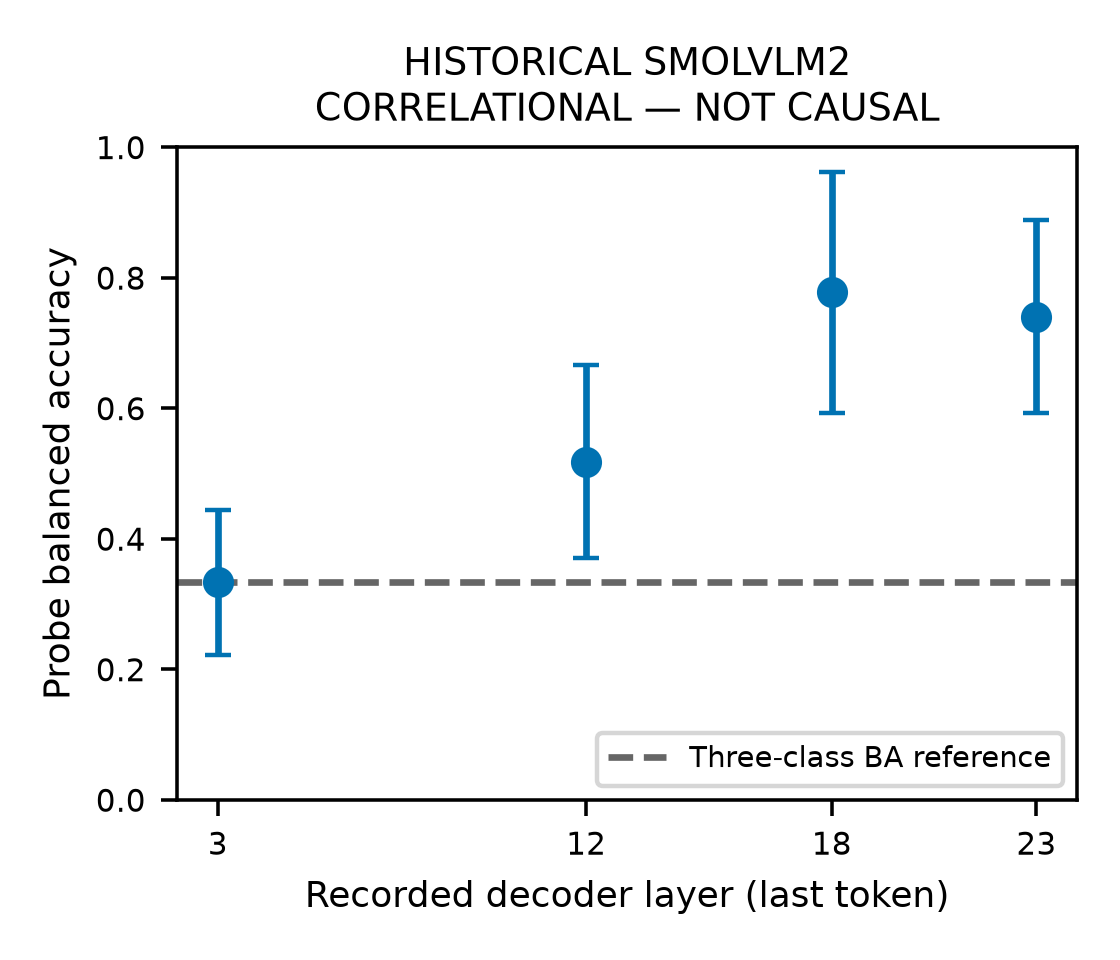
\includegraphics[width=\linewidth]{figures/10_historical_smol_probes.png}
\caption{Historical SmolVLM2 last-token probe BA: layers 3/12/18/23 = 0.333333/0.518519/0.777778/0.740741. External probes used 81 training cases/27 families and 27 validation cases/nine families. Bars retain stored descriptive B=2000 family intervals. Layer/selector/L2 selected on development data. BA independently checked from confusion counts; stored CI endpoints were not independently resampled in this mission. Separate from Qwen.}
\label{fig:10_historical_smol_probes}
\end{figure}
